\documentclass[11pt]{article}

% ==== Paquetes ====
\usepackage[utf8]{inputenc}
\usepackage[spanish]{babel}
\usepackage[T1]{fontenc}
\usepackage{amsmath, amssymb, amsfonts, siunitx}
\usepackage{graphicx}
\usepackage{float}
\usepackage{xcolor}
\usepackage{hyperref}
\usepackage{caption}
\usepackage{subcaption}
\usepackage{geometry}
\usepackage{listings}
\usepackage{tikz}

\definecolor{codegreen}{rgb}{0,0.6,0}
\definecolor{codegray}{rgb}{0.5,0.5,0.5}
\definecolor{codepurple}{rgb}{0.58,0,0.82}
\definecolor{backcolour}{rgb}{0.95,0.95,0.92}

\lstset{
  inputencoding=utf8,
  extendedchars=true,
  literate=
   {á}{{\'a}}1 {é}{{\'e}}1 {í}{{\'i}}1 {ó}{{\'o}}1 {ú}{{\'u}}1
   {Á}{{\'A}}1 {É}{{\'E}}1 {Í}{{\'I}}1 {Ó}{{\'O}}1 {Ú}{{\'U}}1
   {ñ}{{\~n}}1 {Ñ}{{\~N}}1
   {¿}{{?`} }1 {¡}{{!`} }1
}

\lstdefinestyle{mystyle}{
    backgroundcolor=\color{backcolour},   
    commentstyle=\color{codegreen},
    keywordstyle=\color{magenta},
    numberstyle=\tiny\color{codegray},
    stringstyle=\color{codepurple},
    basicstyle=\ttfamily\footnotesize,
    breakatwhitespace=false,         
    breaklines=true,                 
    captionpos=b,                    
    keepspaces=true,                 
    numbers=left,                    
    numbersep=5pt,                  
    showspaces=false,                
    showstringspaces=false,
    showtabs=false,                  
    tabsize=2,
    upquote=true,
    inputencoding=utf8,
}

\lstset{style=mystyle}

\geometry{margin=2.5cm}

% ==== Datos de la tarea ====
\title{IEE3584 - Comunicaciones inalámbricas \\
Tarea 9}
\author{Nicolás Seguel}
\date{Octubre 2025}

\begin{document}
\maketitle

\section*{Problema 18: (15 puntos)}

Considere los presupuestos de enlace del Problema 9.

\begin{enumerate}
    \item (5 puntos) En el caso para el que su colega hizo el cálculo, ¿Cuántas antenas de diversidad MRC en el receptor serían necesarias para aumentar la cobertura a 98\%?
    \item (5 puntos) Para el mismo caso anterior, ¿Qué cobertura se lograría con diversidad de selección pura de orden 4?
    \item (5 puntos) En el caso que su colega no calculó, ¿Es posible lograr cuadrar el presupuesto usando diversidad de algún tipo (transmisor, receptor, selección pura, MRC, ganancias iguales)? Justifique su respuesta.
\end{enumerate}

\subsection*{Solución:}

\begin{enumerate}
    \item La probabilidad de que la SNR instantánea sea menor que un umbral $\gamma_{th}$ en un canal Rayleigh con diversidad MRC de orden $N_r$ está dada por:

    \[
    P_{out}(\Gamma_0, k) = 1 - e^{-\frac{\Gamma_{0}}{\overline{\gamma}}} \sum_{k=1}^{N_r} \frac{\left(\frac{\Gamma_{0}}{\overline{\gamma}} \right)^{k-1}}{\left(k - 1\right)!}
    \]

    De la pregunta 9, se sabe que la SNR media por rama es $\overline{\gamma} = $ dB y el umbral de SNR es $\Gamma_0 = 7.5$ dB. Convirtiendo estos valores a escala lineal:

    \[
    \overline{\gamma} = 10^{\frac{17.5}{10}} \approx 56.23
    \]

    \[
    \Gamma_0 = 10^{\frac{7.5}{10}} \approx 5.62
    \]

    Ahora, para encontrar el orden de diversidad necesario para alcanzar una probabilidad de outage de $P_{out, N_r} = 0.02$, podemos buscar el valor de $N_r$ que satisface:

    \[
    N_r = 1 \implies P_{out, 4} = 1 - e^{-0.1} \sum_{k=1}^{4} \frac{(0.1)^{k-1}}{(k - 1)!} \approx 0.095
    \]

    \[
    N_r = 2 \implies P_{out, 5} = 1 - e^{-0.1} \sum_{k=1}^{5} \frac{(0.1)^{k-1}}{(k - 1)!} \approx 0.0046
    \]

    Por lo tanto, se necesitan al menos 2 antenas de diversidad MRC en el receptor para alcanzar una cobertura del 99.5\%.

    \item La probabilidad de outage para diversidad de selección pura (SC) está dada por:
    
    \[
    P_{out}(\Gamma_0, N_r) = \left(1 - e^{-\frac{\Gamma_{0}}{\overline{\gamma}}}\right)^{N_r}
    \]

    Usando los mismos valores de $\overline{\gamma}$ y $\Gamma_0$ que antes, calculamos la probabilidad de outage para $N_r = 2$:

    \[
    N_r = 2 \implies P_{out, 2} = \left(1 - e^{-0.1}\right)^{2} \approx 0.009
    \]

    Por lo tanto, la cobertura lograda con diversidad de selección pura de orden 2 es aproximadamente $1 - 0.009 = 99.1\%$.

    \item Para el caso no calculado, se tiene una SNR media por rama de $\overline{\gamma} = 1.28$ dB y un umbral de SNR de $\Gamma_0 = 7.5$ dB. Realizamos los cálculos para diversidad MRC y SC:
    
    \[
    N_r = 8 \implies P_{out, 8}^{MRC} = 1 - e^{-4.1879} \sum_{k=1}^{8} \frac{\left(4.1879\right)^{k-1}}{(k - 1)!} \approx 0.0631
    \]

    \[
    N_r = 8 \implies P_{out, 8}^{SC} = \left(1 - e^{-4.1879}\right)^{8} \approx 0.9996
    \]

    En este caso, incluso con 8 antenas de diversidad, la probabilidad de outage para MRC es aproximadamente 6.31\%, lo que cumple con el requisito de cobertura del 90\%. Para SC, la probabilidad de outage es prácticamente 100\%, lo que implica que se necesitarían muchas más antenas para cumplir con el requisito. Por lo tanto, es posible cuadrar el presupuesto usando diversidad MRC, pero no con diversidad de selección pura.
\end{enumerate}

\section*{Problema 21: (20 puntos)}

En un sistema de diversidad de recepción en que cada rama observa desvanecimiento Rayleigh independiente, ¿Qué orden de diversidad es necesario en una transmisión BPSK para que el punto de operación $P_b = 10^{-3}$ sea logrado con menor razón señal a ruido que la misma transmisión sin diversidad en ruido blanco Gaussiano?  

Responda la pregunta para:

\begin{enumerate}
    \item (8 puntos) MRC.
    \item (12 puntos) Selección pura.
\end{enumerate}

\subsection*{Solución}

Calculamos primero la SNR necesaria para alcanzar $P_b = 10^{-3}$ en un canal AWGN sin diversidad. La probabilidad de error para BPSK en AWGN está dada por:

\[
P_b = Q\left(\sqrt{2\gamma}\right)
\]

Despejando para $\gamma$ cuando $P_b = 10^{-3}$:

\[
Q^{-1}(10^{-3}) \approx 2.3267 \implies \sqrt{2\gamma} = 2.3267 \implies \gamma \approx \frac{(2.3267)^2}{2} \approx 2.326 \approx 4.324 \text{ dB}
\]

\begin{enumerate}
    \item Para diversidad MRC, la probabilidad de error promedio para BPSK en un canal Rayleigh, según Goldsmith, está dada por
    
    \[
    \overline{P_b} = \frac{1}{\pi} \int_{0}^{\frac{\pi}{2}} \left( \frac{1}{1 + \frac{\overline{\gamma}}{\sin^2(\theta)}} \right)^{N_r} d\theta
    \]

    Probamos diferentes valores de $N_r$ hasta encontrar el mínimo que satisface $\overline{P_b} \leq 10^{-3}$ con una SNR menor a 4.324 dB. Se encuentra que para $N_r = 4$, la SNR necesaria es aproximadamente 4.03 dB, que es menor que 4.324 dB.

    \item Para diversidad de selección pura (SC), la probabilidad de error promedio para BPSK en un canal Rayleigh está dada por:
    
    \[
    \overline{P_b} = \int_{0}^{\infty} Q\left(\sqrt{2\gamma}\right) f_{\gamma_{SC}}(\gamma) d\gamma
    \]

    Nuevamente, probamos diferentes valores de $N_r$ hasta encontrar el mínimo que satisface $\overline{P_b} \leq 10^{-3}$ con una SNR menor a 4.324 dB. Se encuentra que para $N_r = 5$, la SNR necesaria es aproximadamente 3.590 dB, que es menor que 4.324 dB.

\end{enumerate}

\lstinputlisting[
    style=mystyle,
    language=Python,
    caption={Archivo \texttt{pregunta21.py}: cálculo de SNR para diversidad MRC y SC.}
]{pregunta21.py}

\section*{Problema 22: (15 puntos)}

Un sistema 16-QAM utiliza diversidad de recepción MRC en un canal con desvanecimiento Rayleigh independiente entre ramas. Grafique la probabilidad media de error de símbolo ($\overline{P}_s$) vs. razón señal a ruido media por rama ($\overline{\gamma}$) para diversidad de orden $N_r = 1, \ldots, 8$.

\textbf{Indicación:} Consulte el capítulo 6 del texto de Goldsmith [3] y considere usar integración numérica.

\subsection*{Solución}

La probabilidad media de error de símbolo para 16-QAM con diversidad MRC en un canal Rayleigh está dada por:

\[
\overline{P_s} = \frac{4}{\pi} \left(1 - \frac{1}{\sqrt{M}}\right) \int_{0}^{\frac{\pi}{2}} \left(\frac{3\overline{\gamma}}{(M-1)\sin^2(\theta)} \right)^{N_r} d\theta - \frac{4}{\pi} \left(1 - \frac{1}{\sqrt{M}}\right)^2 \int_{0}^{\frac{\pi}{4}} \left( \frac{3\overline{\gamma}}{(M-1)\sin^2(\theta)} \right)^{N_r} d\theta
\]

Resolviendo numéricamente se tiene:

\begin{figure}[H]
    \centering
    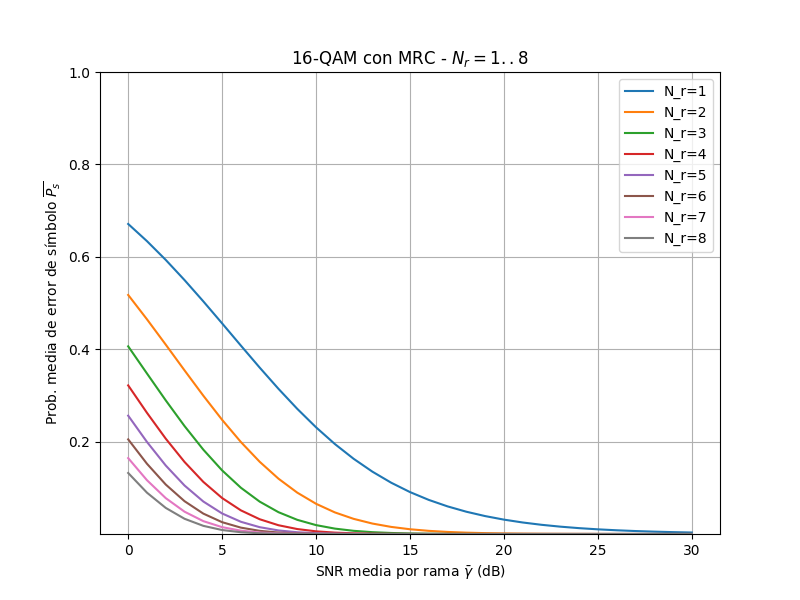
\includegraphics[width= 0.8\linewidth]{fig1.png}
    \caption{Probabilidad de error media por símbolo para diferente número de antenas}
\end{figure}

\lstinputlisting[
    style=mystyle,
    language=Python,
    caption={Archivo \texttt{pregunta22.py}: cálculo y gráfico de probabilidad media de error de símbolo para 16-QAM con diversidad MRC.}
]{pregunta22.py}

\end{document}
